\subsection{Optimal parameters choice}
For a given set of tolerances of the convergence criterion, the paramters that need to be chosen carefully are essentially the inverse power step tolerance and the number of maximum GCG iterations.
\subsubsection{Inverse power step tolerance}
The inverse power step tolerance is one of the biggest bottlenecks of the computational cost of the solver. A careful choice is needed for correct eigenvalues convergence, while mainting the computational cost at bay.
\\From figure \ref{fig:conv_tol}, it's clear that at least a tolerance of $10^{-3}$ is needed for good convergence, while tolerances $\ge 10^{-4}$ stop offering increasing returns, rendering a choice between $10^{-4}$ and $10^{-5}$ an optimal one.
\begin{figure}[H]
    \centering
    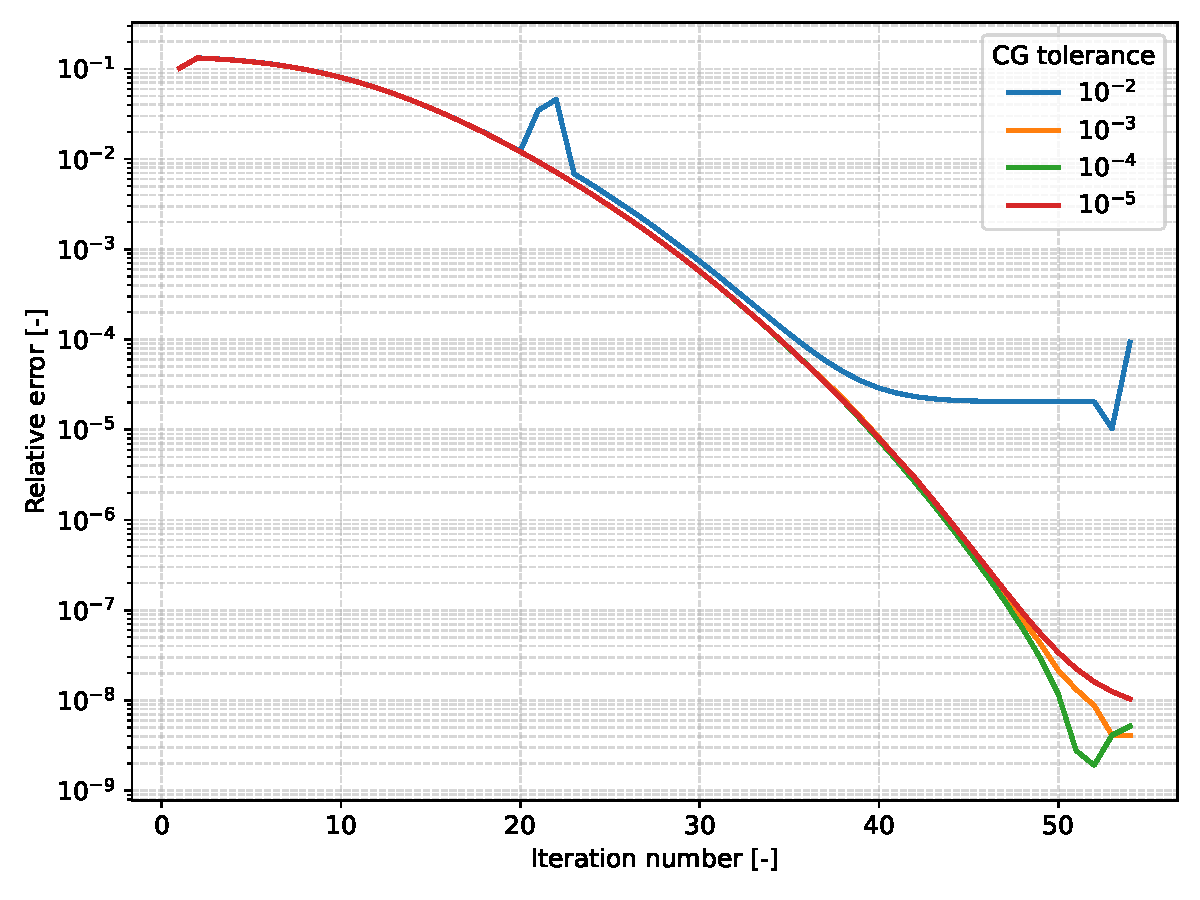
\includegraphics[width=0.9\textwidth]{Images/conv_tol.pdf}
    \caption{HF calculation convergence with varying CG tolerance. $^{16}$O}
    \label{fig:conv_tol}
\end{figure}
\subsubsection{Inner GCG iterations}
The number of inner GCG iterations, here named `inverse power steps` to avoid confusion, is slightly more nuianced than the CG tolerance. One could think that a higher number of iterations would bring to convergence faster since the precision on the eigenalues increases, but this is not the case.
\\In figures \ref{fig:conv_steps_o} and \ref{fig:conv_steps_mg}, the convergence of the HF calculation is plotted for different number of steps, respectively, for the spherical nucleus $^{16}$O and the deformed nucleus $^{24}$Mg. 
\begin{figure}[H]
    \centering
    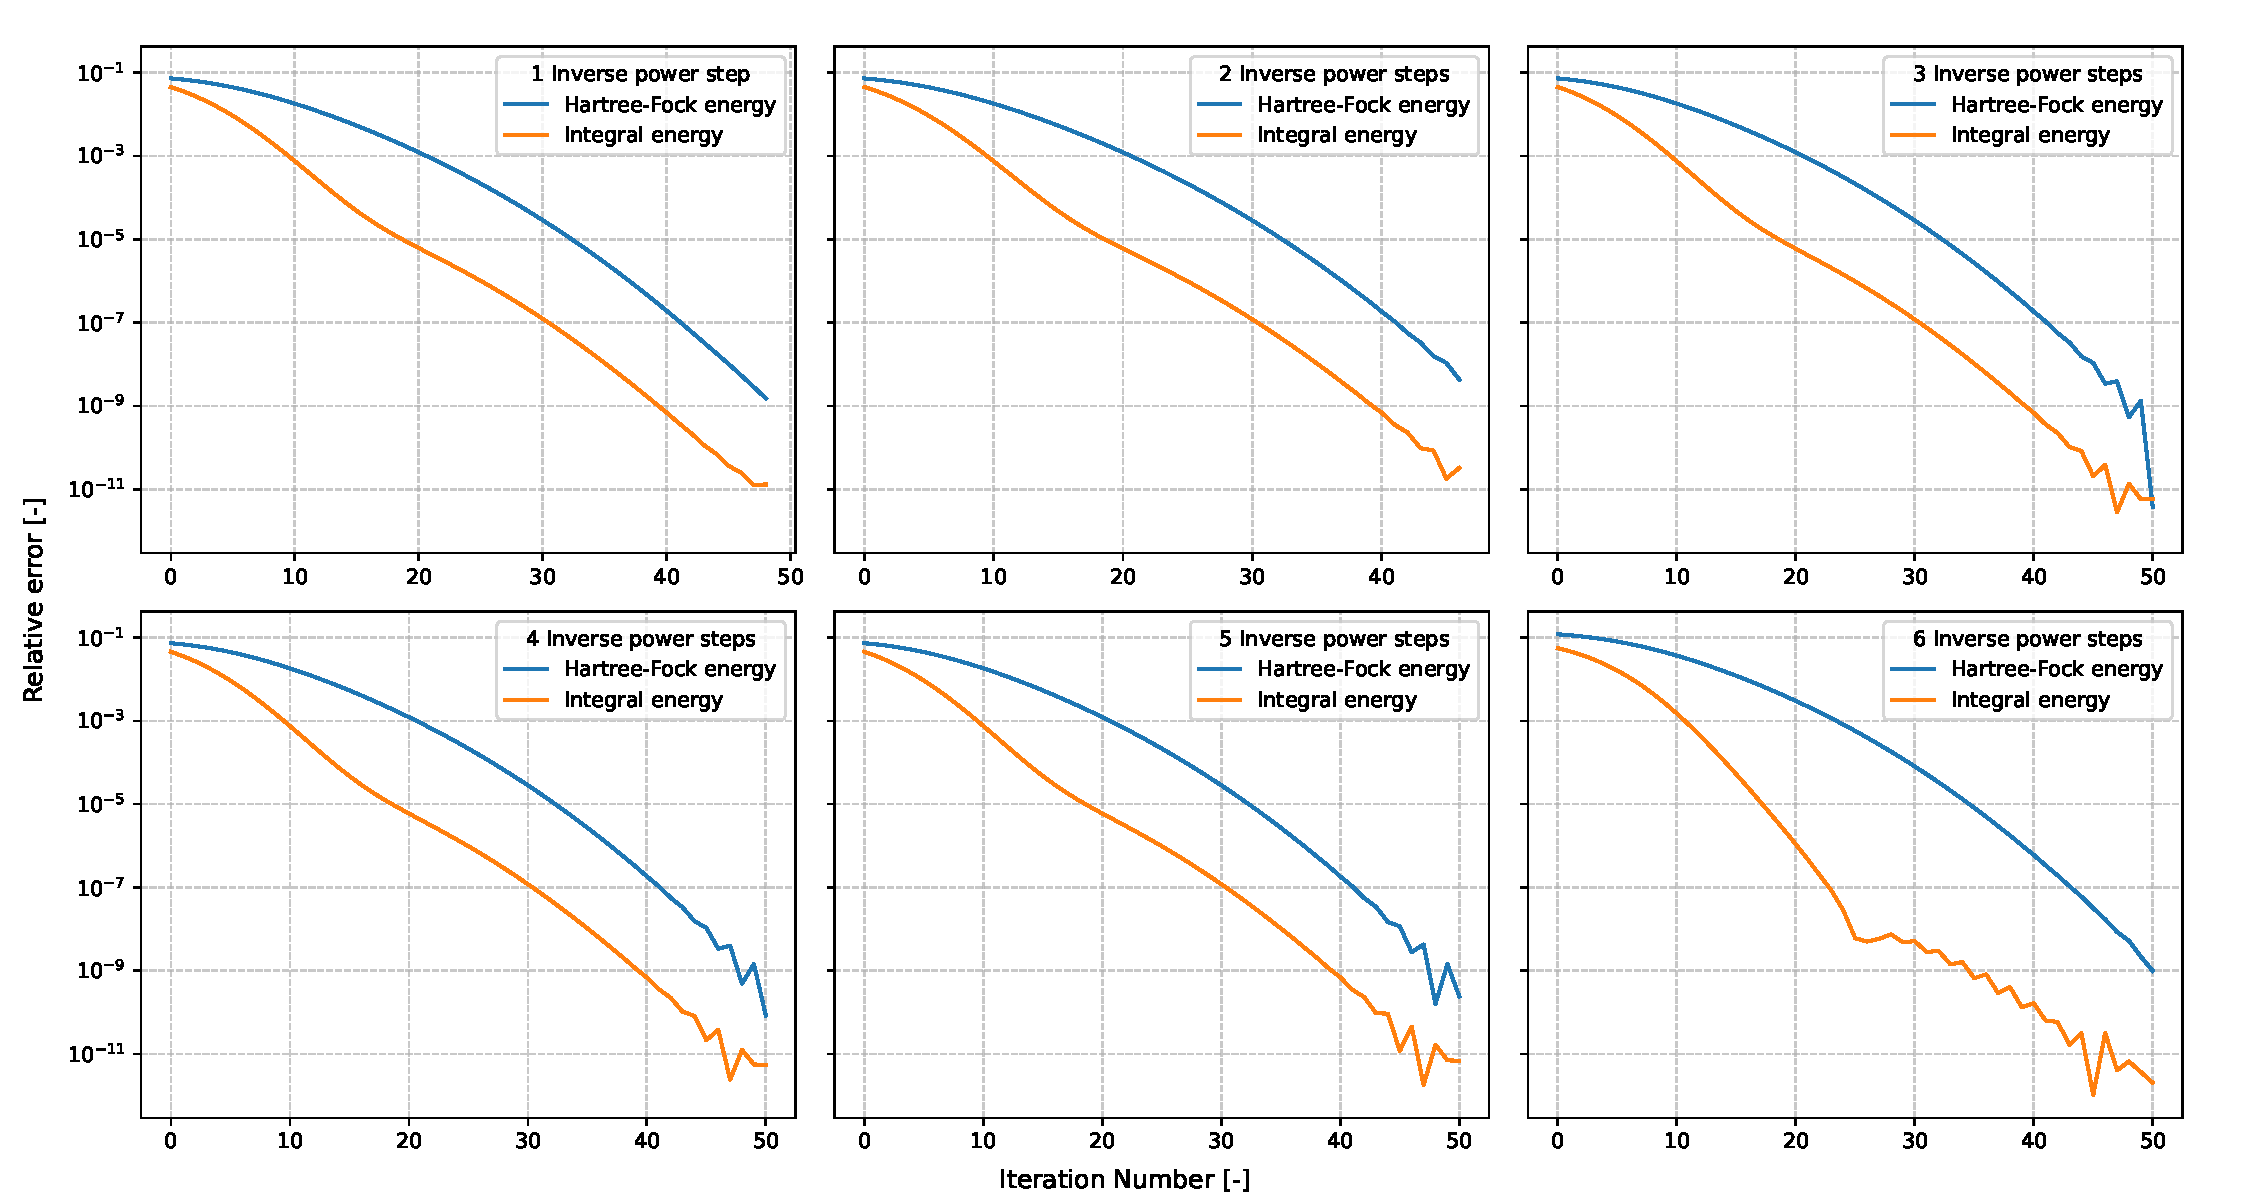
\includegraphics[width=1.0\textwidth]{Images/conv_steps_o.pdf}
    \caption{HF calculation convergence with varying number of inverse power steps for the spherical nucleus. $^{16}$O}
    \label{fig:conv_steps_o}
\end{figure}
\begin{figure}[H]
    \centering
    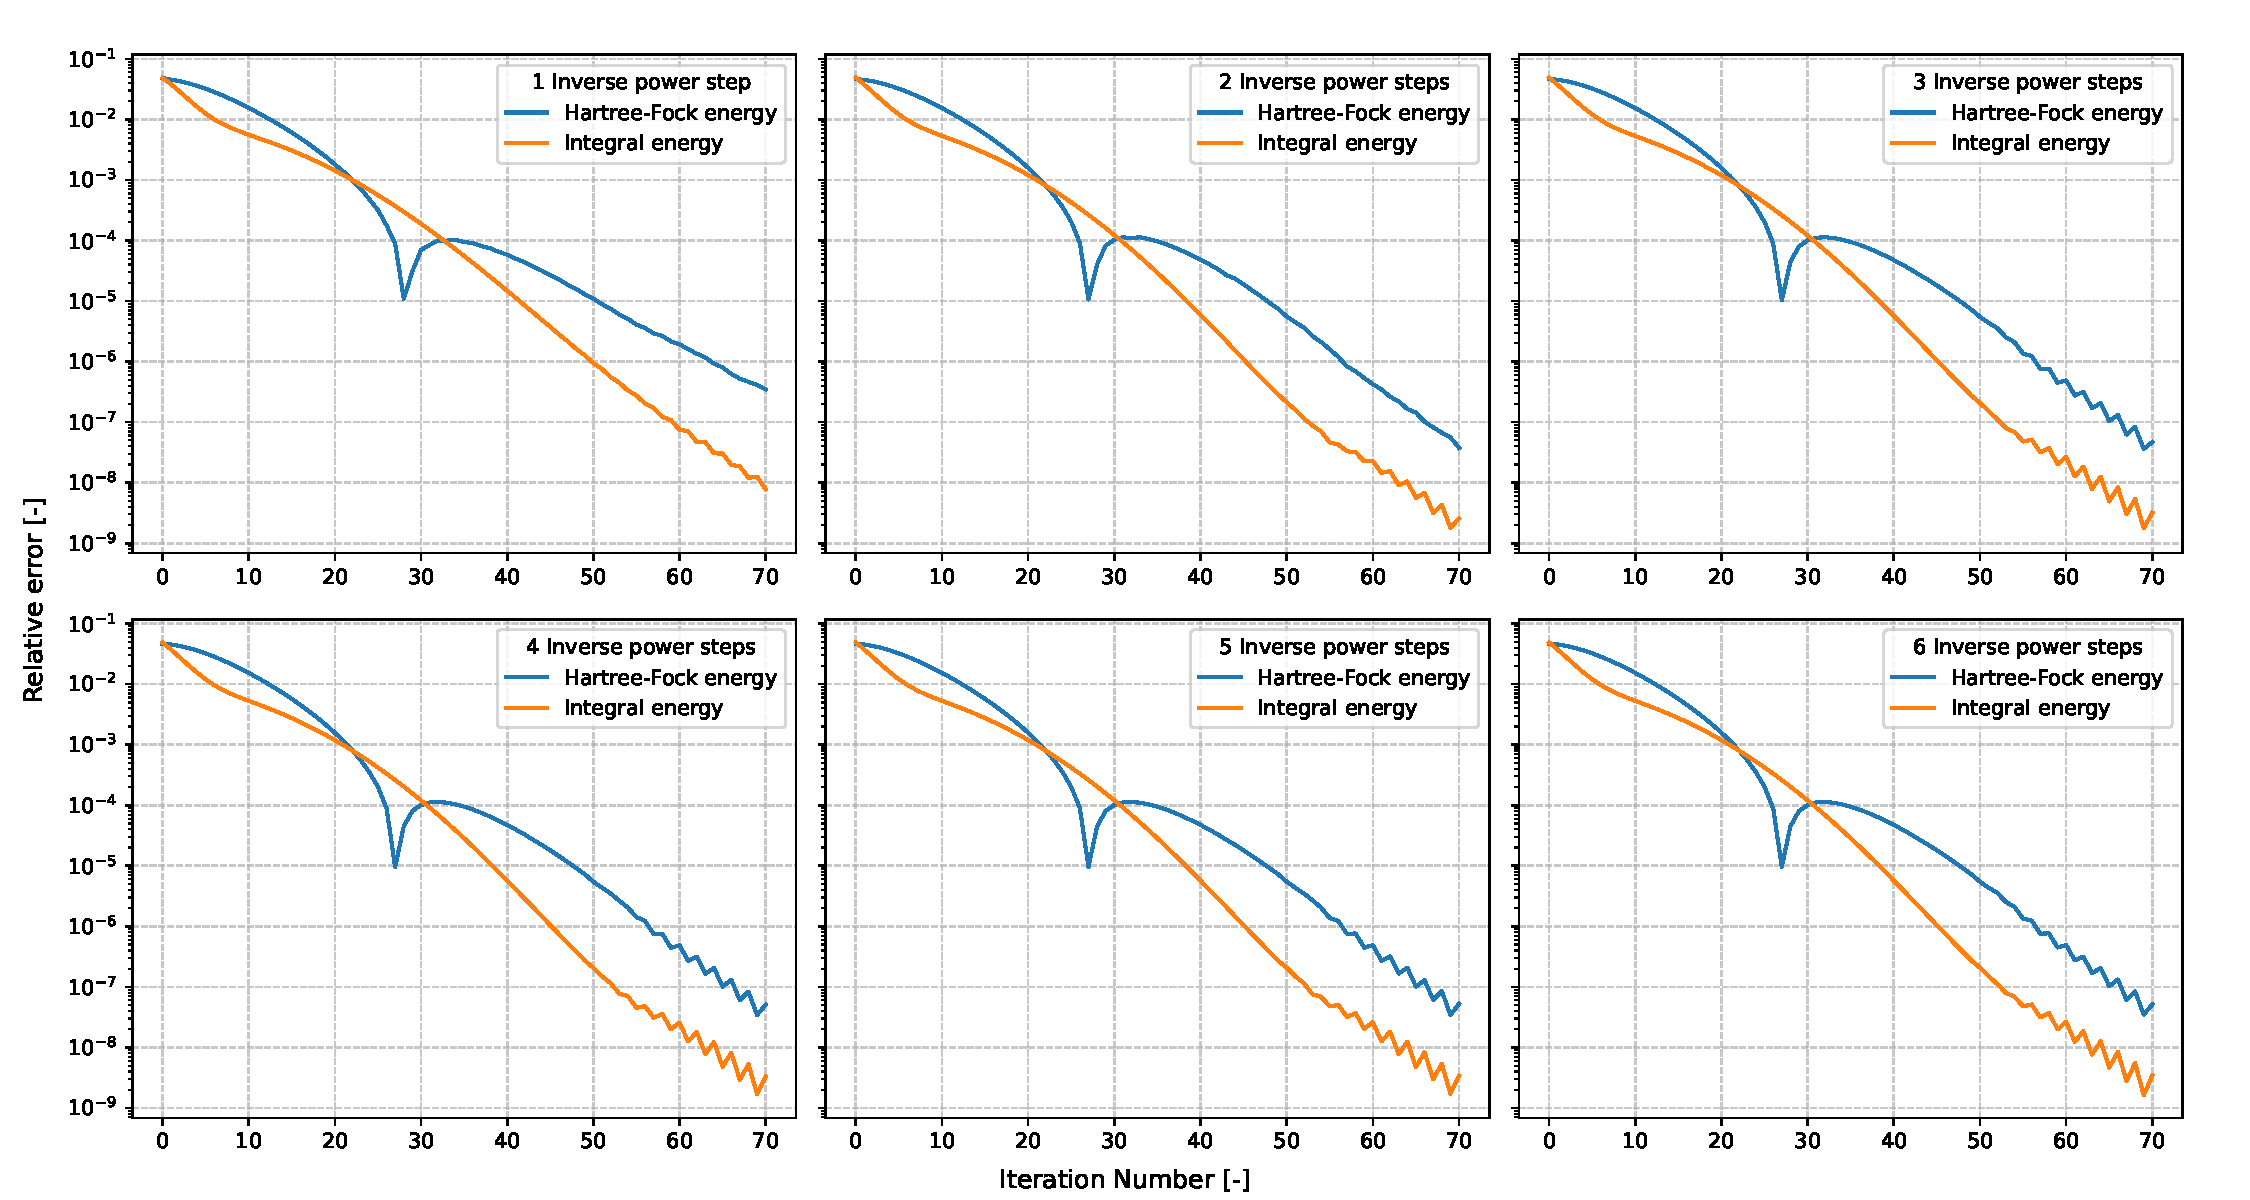
\includegraphics[width=1.0\textwidth]{Images/conv_steps.pdf}
    \caption{HF calculation convergence with varying number of inverse power steps for the deformed nucleus. $^{24}$Mg}
    \label{fig:conv_steps_mg}
\end{figure}
It's evident that in both cases, a steps number greater than $3$ leads to a more unstable convergence, while in the case of the spherical nucleus, just one step is enough to quickly, and safely, reach convergence.
\\This is likely due to the fact that at each HF iteration the hamiltonian changes and a great number of steps leads to solutions too biased towards the current matrix eigenvalues, at the expense of the next iteration; however, in the case of deformed nuclei, due to sharp shape changes at the start of the calculation, just one step may not be enough to sustain the pace at which the Hamiltonian changes, hence the quicker convergence with more steps.



